\documentclass{beamer}
%
% Choose how your presentation looks.
%
% For more themes, color themes and font themes, see:
% http://deic.uab.es/~iblanes/beamer_gallery/index_by_theme.html
%
\mode<presentation>
{
  \usetheme{Warsaw}      % or try Darmstadt, Madrid, Warsaw, ...
  \usecolortheme{default} % or try albatross, beaver, crane, ...
  \usefonttheme{default}  % or try serif, structurebold, ...
  \setbeamertemplate{navigation symbols}{}
  \setbeamertemplate{caption}[numbered]
} 

\usepackage[english]{babel}
\usepackage[utf8x]{inputenc}
\usepackage{graphicx}



\title[Circular Economy]{Complexity Insights into Circular Economy}
\author{J. Broere, C. Moore, J. Raimbault, J. M. Serna, M. Somveille, E. Strombom, L. Sugar, B. Zhu}
%\institute{Where You're From}
\date{July 7, 2016}

\begin{document}



\begin{frame}
  \titlepage
\end{frame}

% Uncomment these lines for an automatically generated outline.
%\begin{frame}{Outline}
%  \tableofcontents
%\end{frame}



\begin{frame}{The Circular Economy}

\begin{figure}
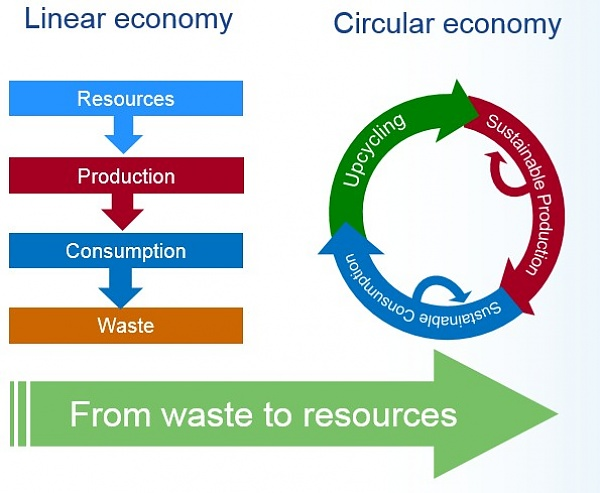
\includegraphics[width=0.8\textwidth]{CE.jpg}

\end{figure}

\end{frame}



\begin{frame}{Why use complexity science?}

\begin{itemize}
\item `Closing the loop' mechanisms
\item Multiple interacting actors 
\item Multiple organizational levels
\item Interdependence
\item Optimizing waste flows
\end{itemize}

% Commands to include a figure:
%\begin{figure}
%\includegraphics[width=\textwidth]{your-figure's-file-name}
%\caption{\label{fig:your-figure}Caption goes here.}
%\end{figure}


\end{frame}



\begin{frame}{Model}

\textit{Simple combination of niche and spatial interaction model as an ABM}

% Q : references here ?

\medskip

\textbf{Setup}

\textbf{Evolution}




\end{frame}

\begin{frame}{Picture of the Model}

\begin{figure}
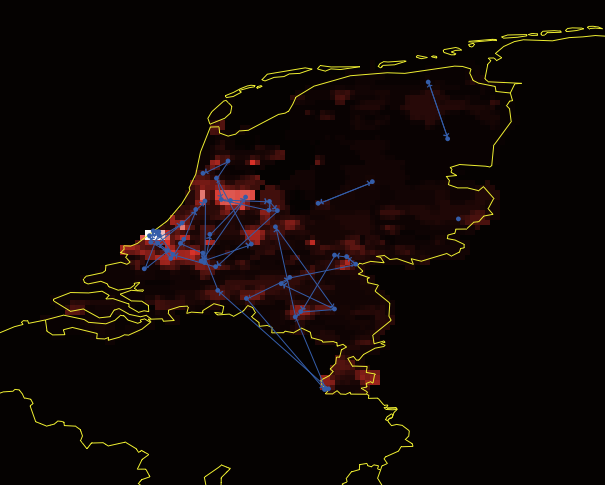
\includegraphics[width=0.8\textwidth]{CENL.png}
\end{figure}

\end{frame}

\begin{frame}{Results}

\end{frame}

\begin{frame}{Perspectives}

\begin{itemize}
\item Test on:
\begin{itemize}
\item Existing maps and infrastructures
\item Use data to calibrate the model
\end{itemize}

\item Open source monitoring
\item Insights into the `waste market'

\end{itemize}
\end{frame}




%%%%%%%%%%%%%%%%%%%%%
%% Reserve slides
%%



\begin{frame}{Reserve Slides}
  \Huge \centering \textit{Reserve slides}
\end{frame}



\begin{frame}{Indicators (uniform spatial distribution)}
\begin{figure}
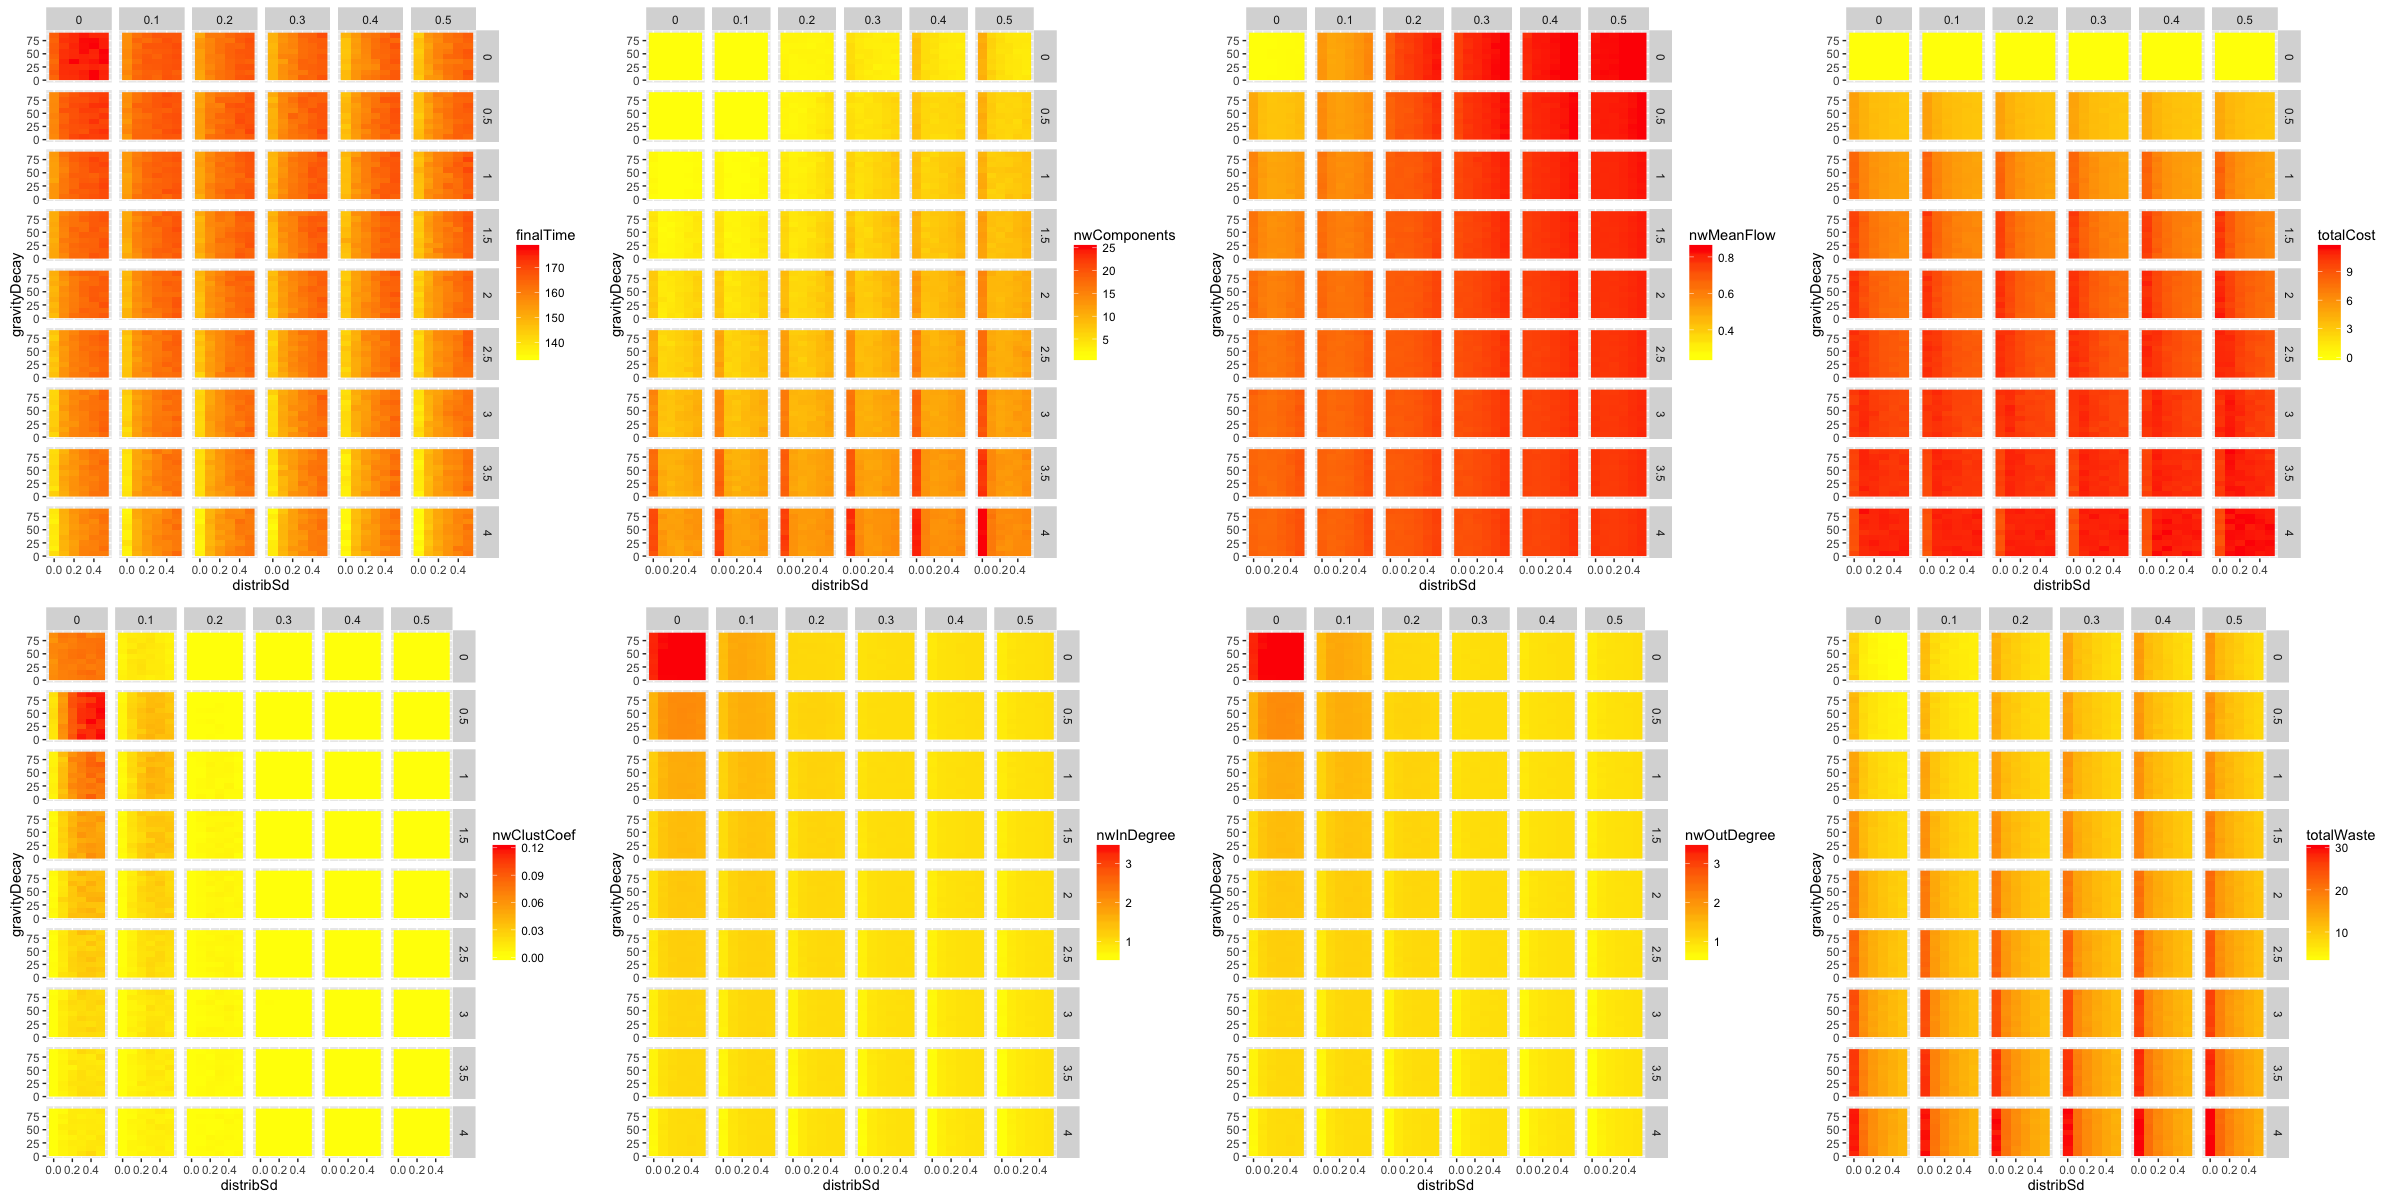
\includegraphics[width=\textwidth]{figures/heatmap_indics}
\end{figure}
\end{frame}


\begin{frame}{Pareto front (uniform spatial distribution)}
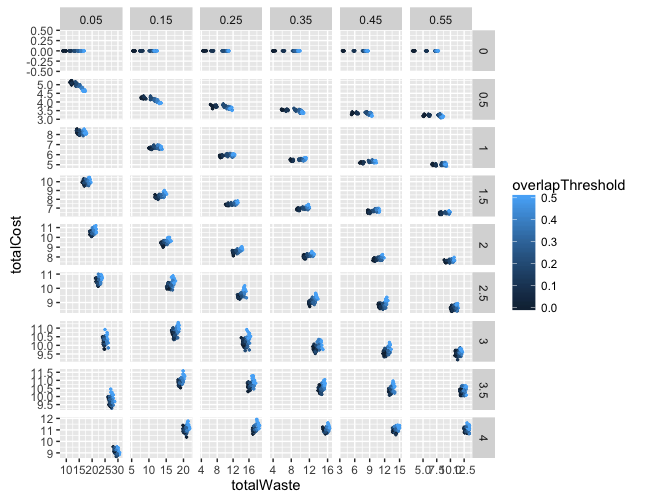
\includegraphics[width=\textwidth]{figures/pareto_wasteCost_overlapThreshold}
\end{frame}




\end{document}
